\documentclass[conference,compsoc]{IEEEtran}

% *** CITATION PACKAGES ***
%
\ifCLASSOPTIONcompsoc
  % IEEE Computer Society needs nocompress option
  % requires cite.sty v4.0 or later (November 2003)
  \usepackage[nocompress]{cite}
\else
  % normal IEEE
  \usepackage{cite}
\fi

\usepackage{graphics}
\usepackage{graphicx}
\usepackage{amsmath}
\usepackage{algorithm, algorithmic}
\renewcommand{\algorithmicrequire}{\textbf{Input:}}
\renewcommand{\algorithmicensure}{\textbf{Output:}}
\usepackage{array}
\usepackage{url}
% correct bad hyphenation here
\hyphenation{op-tical net-works semi-conduc-tor}


\begin{document}
\title{Project 4: Support Vector Machine}

% author names and affiliations
% use a multiple column layout for up to three different
% affiliations
\author{\IEEEauthorblockN{Yuejian Mo  11510511}
\IEEEauthorblockA{Department of Biology\\
Southern University of Science and Technology\\
Email: 11510511@mail.sustc.edu.cn}}

% make the title area
\maketitle

\IEEEpeerreviewmaketitle

\section{Preliminaries}

Support vector machine, are supervised learning models with associated learning
algorithms that analyze data used for classification and regression analysis.
Given a set of training examples, each marked as belonging to one or the other
of two categories, an SVM training algorithm builds a model that assigns new
examples to one category or the other, making it a non-probabilistic binary
linear classifier.\cite{1} If the dataset are points in space, we can find out
an gap separate dataset into two part by using SVM.

\begin{figure}[ht!]
\centering
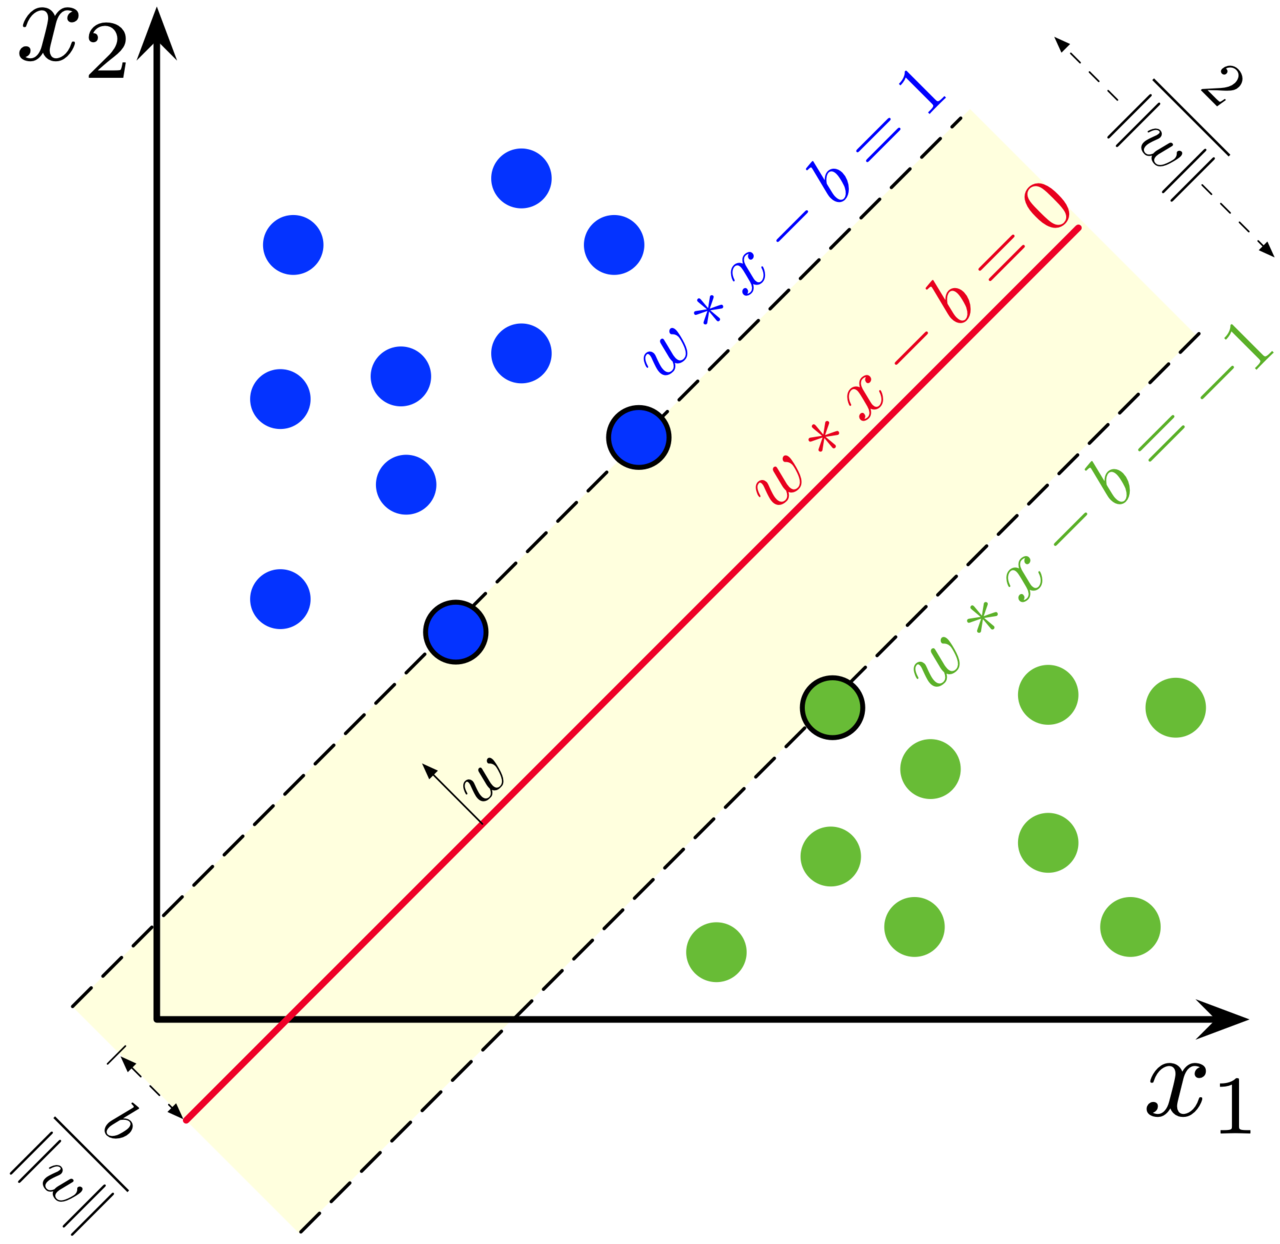
\includegraphics[width=0.65\linewidth]{1280px-SVM_margin.png}
\caption{Separate data points into two part using SVM(from Larhmam) 
	\label{SVM demostrains}}
\end{figure}

The original SVM algorithm was invented by Vladir N. Vapnik and
Alexey Ya. Chervonenkis in 1963. During the development, SVM are able to deal
with more tasks. SVM are used in text and hypertext categorization,
classification of images, hand-written characters recognition and proteins
classification.

In this project, I use SVM with random gradient descent to classify training
data almost correctly. 

% Add figure here

\subsection{Software}
This project is written by Python 3.7 with editor Vim. Numpy, os, time,
random, sys and argparse library are used.

\subsection{Algorithm}
Model question with SVM. To optimal time cost and current of solution, random
gradient descent is used.

\section{Methodology}
Training data is ....

SVM is modeled as ...

random ....

Training set contain 1334 sample, and each sample contain 10 features and 1
label. With the help of other mathematical tools, training data show that
it can be classified in linear model. So, SVM model is used as training
model.

For most common and basic SVM(Figure 1), linear SVM uses two parallel vector
$w\cdot{x}-b=1$
and $w\cdot{x}-b=-1$ to separate dataset $x$ into two parts, where $x$ is
$m*n$ matrix with $n$ training samples of $m$ features, $w$ is a $m$ dimension
vector of SVM parameters and $b$ also is parameter of SVM. The rule is that gap
between two support vector don't exist any points expect of on the vectors.
To optimal correctness of classification, enlarging the distance
$\frac{2}{||w||}$ between two support vector is one of method. It belong to
convex optimization problem as following:

$${min}_{w,b}\frac{||w||^2}{2}$$
$$s.t. y_i((w\cdot{x_i})+b) \le1, i=1,...,n$$

To train data, we use loss function(also called cost function) to measure the
difference between SVM's prediction and actual labels. Each training, SVM try
to decrease the value of loss function. 

$$ L(w,b)=\sum^n_i=1 max(0, 1-y_i((w_i, x_i)+b)) $$

Then Gradient descend is used to update the feature weight matrix $w$. Each
training, gradient descend promote loss function decrease by moving to
opposite direction of gradient.

$$ w = w -\alpha\frac{dL(w,b)}{dw}$$
$$ \frac{dL(w,b)}{dw} = $$


Finally, the seed required for IMP is generated by a natural greedy algorithm.
Each time, a node with highest influence will added to a seeds set. This empty
seed set will fill with $k$ node, where $k$ is given from outside.

\subsection{Representation}
Some main data are maintain during process: \textbf{time\_budget},
\textbf{node\_num}, \textbf{graph\_cp}, \textbf{graph\_pc}, \textbf{incoming}.
Others data would be specified inside functions.

\begin{itemize}
  \item \textbf{x}: Numpy matrix to store input data.
  \item \textbf{y}: 1-d numpy matrix of label of input data.
  \item \textbf{w}: 1-d numpy matrix of weight and bias of SVM parameters.
\end{itemize}


\subsection{Architecture}
Here list main functions of \textbf{SVM.py} in given code:
\begin{itemize}
    \item \textbf{init}: load train data to $x$, $y$; load time limit; initialize
	    parameter matrix $w$.
    \item \textbf{cal\_sgd}: Update $w$ using gradient descent.
    \item \textbf{train}: Train $w$ from train data data $x$, $y$.
    \item \textbf{predict}: Predict label of test data
    \item \textbf{\_\_main\_\_}: Main function
\end{itemize}

The \textbf{SVM.py} is executed locally.

\subsection{Detail of Algorithm}
Here describes some vital functions.
\begin{itemize}
    \item \textbf{init}: load train data and initial parameters
    \begin{algorithm}[H]
     \caption{int}
     \begin{algorithmic}[1]
     \renewcommand{\algorithmicrequire}{\textbf{Input:}}
     \renewcommand{\algorithmicensure}{\textbf{Output:}}
     \REQUIRE $input\_file\_name, time\_limit$
     \ENSURE $x, y, w, cycle$
     \STATE open $input\_file\_name$ as $file$
     \STATE set $data$
     \FOR {each line in $file$}
          \STATE split line, then package and append line info to $data$
     \ENDFOR
     \STATE transform set $data$ to matrix $x$
     \STATE $y \leftarrow x[:,-1]$ 
     \STATE $x[:, -1] \leftarrow 1$
     \STATE initialize $w$ with length of $x[:, -1]$ and value of 0
     \STATE $cycle$
     \RETURN $x, y, w, cycle$
     \end{algorithmic}
   \end{algorithm}

   \item \textbf{cal\_sgd}:Update $w$ using gradient descent
     \begin{algorithm}[H]
     \caption{cal\_sgd}
     \begin{algorithmic}[2]
     \renewcommand{\algorithmicrequire}{\textbf{Input:}}
     \renewcommand{\algorithmicensure}{\textbf{Output:}}
     \REQUIRE $xi, yi, w, ratio, learn\_speed$
     \ENSURE $w\_next$ 
     \IF {$yi*(\cdot{xi}{w}) < 1$}
	     \STATE $w\_next = w - ratio*(learn\_speed*w - yi*xi)$
     \ELSE
	     \STATE $w\_next = w - ratio*learn\_speed*yi$
     \ENDIF
     \RETURN $w\_next$
     \end{algorithmic}
     \end{algorithm}

  \item \textbf{train}: Train $w$ with data $x, y$
    \begin{algorithm}[H]
     \caption{train}
     \begin{algorithmic}[3]
     \renewcommand{\algorithmicrequire}{\textbf{Input:}}
     \renewcommand{\algorithmicensure}{\textbf{Output:}}
     \REQUIRE $x, y, w, cnt, learn\_speed$
     \ENSURE  $w$
     \STATE $t \leftarrow 0$
     \WHILE{ running time don't exceed ordered time}
	     \STATE reorder $x$ and $x$ in the same time
	     \STATE $loss \leftarrow 0$ 
	     \STATE $t \leftarrow t+1$
	     \STATE $1//(t*learn\_speed)$
	     \FOR{ each line $x_i$ and $y_i$ in training data}
	          \STATE $w = cal\_sgd(x_i, y_i, w, ratio, learn\_speed$
	     \ENDFOR
     \ENDWHILE
     \RETURN $w$
     \end{algorithmic}
     \end{algorithm}
 
 \item \textbf{predict}: Predict the label of test data
     \begin{algorithm}[H]
     \caption{predict}
     \begin{algorithmic}[4]
     \renewcommand{\algorithmicrequire}{\textbf{Input:}}
     \renewcommand{\algorithmicensure}{\textbf{Output:}}
     \REQUIRE $test\_file, w$
     \ENSURE  $label\_set$
     \STATE open $test\_file$ as $file$
     \STATE create set $test\_data$
     \FOR {each line in $file$}
          \STATE split line, then package and append line info to $test\_data$
     \ENDFOR
     \STATE transform set $test\_data$ to matrix $test\_set$
     \STATE $test\_set[:, -1] \leftarrow 1$
     \STATE create $label\_set$
     \STATE $label\_set \leftarrow  sgn(\cdot{test\_set}{w})$
     \RETURN $label\_set$
     \end{algorithmic}
     \end{algorithm}
 

\end{itemize}


\section{Empirical Verification}
Empirical verification is verified offline with given data set. We do the 
OJ system. $ISE.py$ almost pass all
dataset with reasonable bias. $IMP.py$ only was test with network-5-IC and
provide reasonable seeds set.

\subsection{Design}
SVM classify data at less 90 percent robust.

Random gradient return in reasonable time than simple gradient down algorithm.

Independent cascade model return reasonable influence is small graph and big graph.
But Linear Threshold model return less reasonable due with large graph. Finally,
I found my code would added some element repeatedly result in larger bias.

For hill greedy, because I just evaluate once, it produce seeds set fast. In
small graph, which produce seeds in 65 percent effect. But
Not optimal seeds are produced every time.

\subsection{Data and data structure}
For the convenience, matrix are used widely to store train set, test set and
features matrix.

\subsection{Performance}
Following table show different performance with different parameters. Offline
test perform at Fedora 29 with $Intel^{®}$ Xeon(R) CPU E5-1680 v3@3.20GHz and
32GiB memory.

\begin{center}
   \begin{tabular}{| l | l | l |}
   \hline
    Dataset             &Run Time(s)   &Result   \\ \hline
    network-seeds-IC     & 23.23        & 5.015  \\
    network-seeds-LT     & 23.23        & 5.015  \\
    network-seeds2-IC    & 23.24        & 30.47  \\ 
    network-seeds2-LT    & 57.79        & 37.03  \\
    NetHEPT-5seeds-LT    & 58.55        & 341.9  \\
    NetHEPT-5seeds-IC    & 27.87        & 276.3  \\
    NetHEPT-50seeds-LT    &         &   \\
    NetHEPT-50seeds-IC    & 27.87        & 1003  \\
    network-5-IC         & 0.73         & 19.45  \\
   \hline
   \end{tabular}
\end{center}
% Table of difference problem

\subsection{Result}
Best model classify data set at 99.6 percent of correctness.

\subsection{Analysis}
% Analysis different parameter's results
Because natural Hill Greedy is kind of greedy algorithm without heuristics, most
of solutions are not optimal. During using adjacent list rather than adjacent
matrix, space cost is more lower than $O(n^2)$. Because every point only is
evaluate once, only less time it cost. Total, no more than $O(n^2)$ is required.

\section*{Acknowledgment}
Thanks TA Yao Zhao who explain question and provide general method to solve it.
And I also thanks for Kebing Sun discuss and share the idea about algorithm.

\bibliographystyle{IEEEtran}
\begin{thebibliography}{1}
\bibitem{1}
Wikipedia
\end{thebibliography}

% that's all folks
\end{document}


